% chap2.tex (Definitions)

\chapter{Smart Grid and PowerTAC Competition}

In this chapter, I will describe the smart grid \cite{fang2012smart} and Power TAC \cite{ketter2013power}.

\section{Traditional Electricity Distribution and Consumption System}
In traditional power grids, there are three subsystems electricity generation, transmission, and distribution \cite{fang2012smart}. In electricity generation subsystem, the generator rotates a turbine in a magnetic field which generates electricity. The turbine rotates through the power of kinetic energy of water falling from a waterfall or a river with strong current, or from the energy of nuclear power plant, or energy received from burning coal or oil. Traditional energy generation system then transmits the electricity through transmission grid and electricity gets distributed through the distribution grid. This generation system is one way meaning a the electricity flow occurs from source node to consumption node only.



\section{Smart Grid}
In contrast to the traditional electricity generation system, Smart Grid are two-way \cite{fang2012smart}. So, any node in the distribution grid can produce electricity and push it to the distribution grid if necessary. The NIST report \cite{fang2012smart} states that the SG would make the electricity generation and supply robust against generator or distribution node failure, use renewable energy widely and efficiently, reduce greenhouse gas emission, reduce oil consumption by encouraging usage of electric vehicles, it will give customers more freedom to choose among energy sources. Smart grids will encourage usage of the electric vehicle as these vehicles have the ability to store power in a battery and transmit the power to the distribution grid if there is a necessity. The major challenge with the usage of renewable energy is it is uncertain. This uncertainty causes the ability to predict how much energy the SG can produce in a future time slot hard. The success of SG will need efficient methods to predict energy production \cite{potter2009building}.


\section{Smart Grid and Renewable Energy}
One of the major focus of Smart Grid will be using renewable energy. There are challenges involved with using this abundant source of energy \cite{richter2012transitioning}. People are already showing strong motivation to use renewable energy as indicated by the statistics that 20\% of total energy is from the renewable sources which are second after coal 24\%. Consumers are using renewable energy due to economic reward and environmental concern. A major challenge with renewable energy is the amount of the energy produced is greatly variable. Since the energy produced is volatile there must be a storage mechanism that balances out the surplus energy. The usage of rechargeable electric vehicles might serve the purpose of storage. Accurate prediction of the renewable energy might enable the electric car users to absorb surplus energy and push it back to the grid in peak hours if necessary. 


\section{Power TAC System}

Power Trading Agent Competition (Power TAC) \cite{ketter2013power}, \cite{ketter20162016}, is a low-risk system that simulates a smart grid based energy system. This simulation system models a competitive and liberal energy trading market. The power TAC simulation has several components such as wholesale market, brokers, customers, distribution utility and weather service \cite{ketter20162016}. The brokers publishes tariff plans for electricity consumers and producers. It then buys electricity from the wholesale and balancing market to meet customers need. The system is trained on customers behavior of past years and uses real weather data. The following sections give a brief explanation of each component of the Power TAC. Figure \ref{fig:simulation-environment}  shows a block diagram of the components of the powerTAC simulation environment.
%advantage 

\subsection{Broker}

In Power TAC system, participants implement their broker logics. Here are the list of actions that a broker can take in Power TAC simulation -
\begin{itemize}  
\item At any hour of the simulation, a broker can publish a new tariff. Each tariff is targetted to a specific category of the customers. The tariffs contain information about which category of customers it is targetted, expiration date of the tariff, signing bonus, penalty for early withdraw and rate of periodic payment. 
\item At any moment of time, a broker can modify its published tariffs. It can adjust payment rates and withdraw penalty. The broker can also revoke a tariff that is not profitable.
\item To meet customer's demand, a broker takes part in the electricity auction in the wholesale market. There, it specifies how much energy it needs and how much it is ready to pay for. Based on the asks and bids from other brokers in the simulation, the broker's bid may or may not get cleared. 
\end{itemize}

At any moment of time the brokers are aware of the following information - 
\begin{itemize}  
\item Participating brokers in the simulation 
\item Customers present in the simulation. 
\item Bootstrap data of customers and wholesale market.
\item Published tariff in the simulation.
\item Information about tariff modification or revocation
\item Wholesale market clearing prices of last time slot.
\item Energy transaction information of subscribed customers.
\item Transaction of balancing market.
\item Current bank balance of itself.
\end{itemize}


\subsection{Customers}
A customer represents an entity that buys energy from the brokers. A customer has the following attributes -
\begin{itemize}  
\item An unique name. 
\item Number of individuals it represents. This number can range from one to several thousands. 
\item A power type that specifies which category of customers (producer or consumer) does it fall into. Producer and consumer categories have several subcategories. 
\end{itemize}

A customer can take the following actions during a simulation - 
\begin{itemize}  
\item Evaluate available tariffs in tariff market.
\item Subscribe or abandon a tariff. Customers try to maximize their economical gain so if there is a lucrative tariff in the market, a customer might try to subscribe to it.
\item Generate meter reading based on produced or consumed energy. The system then sends this meter reading to the broker it subscribed to. 
\item Customers with demand shifting capabilities can shift their demand to favorable time slot.
\end{itemize}
 

\subsection{Weather Service}
The weather service broadcasts weather forecast of future hours and weather report of current hour to the brokers. The weather report contains information such as wind speed, cloud cover, temperature, day of week and month of week. Power TAC uses real weather data from the past that makes the simulation more realistic. Brokers can use these information to forecast demand for the weather sensative consumers. The weather information also makes it possible to forecast about renewable energy producers.

\subsection{Markets and Distribution Utility}

There are three different types of markets in Power TAC simulation, namely, wholsale market, tariff market and balancing market. The wholesale market is the bidding place for buying energy. Bulk energy producers and brokers take part in the wholesale market auction. Brokers can submit their bids for 24 future timeslots in the wholesale market by specifying the price it is prepared to pay. If the bid was successful, the broker receives its desired amount by paying the money. At each time slot, the system notifies the broker about the wholesale market clearing prices. Brokers publish their tariff plans in the tariff market. A tariff holds information about the pricing of the energy. Customers, upon analyzing available tariffs, subscribe to their mostly suited tariff plan. Balancing market represents the market from where the broker can buy energy in case of emergency. For example, if a broker has bought less amount of energy for a given timeslot and it finds it needs more energy then it can buy the necessary amount of energy from the balancing market. Usually, the balancing market transactions are costly for brokers than the wholesale market.

The distribution utility has two main objective. First, it supplies energy to the consumers from whole sale market and from the renewable producers. Secondly, it works as a default broker that publishes default tariffs at the start of the game. This makes sure no customer is ever out of energy. Other brokers are supposed to publish lucrative tariffs to attract customers.


\begin{figure}[h]
  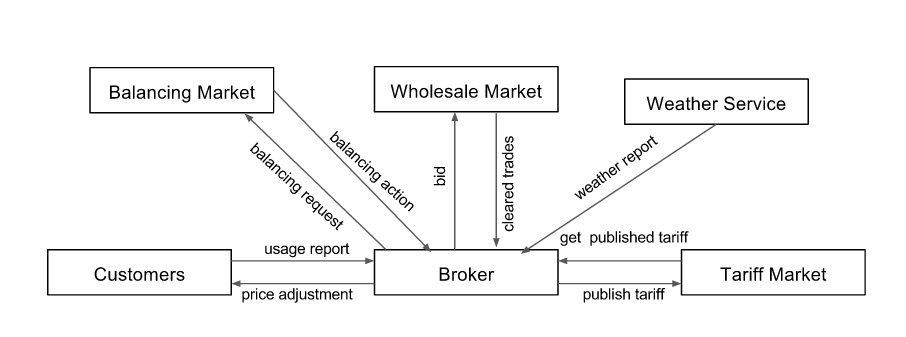
\includegraphics[width=\linewidth]{simulation-environment.png}
  \caption{PowerTAC simulation environment.}
  \label{fig:simulation-environment}
\end{figure}

\section{Importance of Accurate Demand Forecasting in Power TAC}
A broker has to make bids and asks in the wholesale market. The amount of electricity it asks depends on the demand forecast of its subscribed customers. If the broker fails to make accurate demand forecast, it will not be able to ask for proper amount of electricity. So it will end up asking more or less energy than the required amount in the wholesale market. In this case, the broker will have to buy energy from the balancing market in a higher price or has to sell surplus energy in a lower rate. As a result, it will face monetary losses. This unwanted scenario can be avoided through demand forecasting as accurate as possible. This thesis investigates ways to find a better demand forecasting mechanism.


%%% Local Variables: 
%%% mode: latex
%%% TeX-master: "thesis"
%%% End: 
